\section{PS4b: StringSound}\label{sec:ps4b}
\graphicspath{{ps4b}}
\subsection{Discussion:}\label{sec:ps4b:disc}
   This Project produces sound using the SFML library <Audio>, Where we produces notes by using our keys. We utilize the ps4a CircularBuffer in this project.
   Basic motto of this project is to create a simulation of guitar plucking, but as I wanted to do extra credit, I made a Piano simulation note, It is not accurate but close.
   Main thing in this project is using the Karplus-Strong algorithm.

\subsection{Key algorithms, Data structures and OO Designs used in this Assignment:}

The Vector is used for the samples and also creating a sound buffer and holding the sounds bpm. Basic switch method is used for taking the inputs of keys and sending them to calculate the frequency and return with a audio. There are much use of new functions in creating this assignment.

\subsection{Images used:}
\begin{figure}[h]
   \centering
    
\includegraphics[width=0.4\textwidth]{ps4b/backg.jpg}
    \caption{Jazz Background}
    \label{fig:bgps4b}
\end{figure}


\subsection{What I accomplished :}

I accomplished producing piano sounds by altering the frequency. It is an amazing project to create our own instrument using C++.

\subsection{What I already knew :}

I knew how to implement few math functions as well as basics of the SFML.

\subsection{What I learned :}
I learnt how the frequency can be use to create different instruments. I understood how to take the sample inputs from keyboard and produce sound.
\subsection{Challenges :}
Finding out the right frequency and implementing of the samples by reading from the keys was difficult challenge to me.

\subsection{Codebase}\label{sec:ps4b:code}

\textbf{\colorbox{pink}{Makefile}} \newline \textbf{This Makefile contains the lint and is extension of the PS4a Makefile.}

\lstinputlisting[language=Make]{ps4b/Makefile}

\textbf{\colorbox{pink}{KSGuitarSim.cpp}} \newline \textbf{This is the main file where the Samples are taken and window is drawn as well as where takes inputs from keyboard and produces sound.}
\lstinputlisting{ps4b/KSGuitarSim.cpp}

\newpage
\textbf{\colorbox{pink}{StringSound.h}} \newline \textbf{The initialization of the StringSound methods and variables.}
\lstinputlisting{ps4b/StringSound.h}

\textbf{\colorbox{pink}{StringSound.cpp}} \newline \textbf{The frequency is blent in and produces the sound required according to the frequency.}
\lstinputlisting{ps4b/StringSound.cpp}


\subsection{Output:}
\begin{figure}[h]
   \centering
    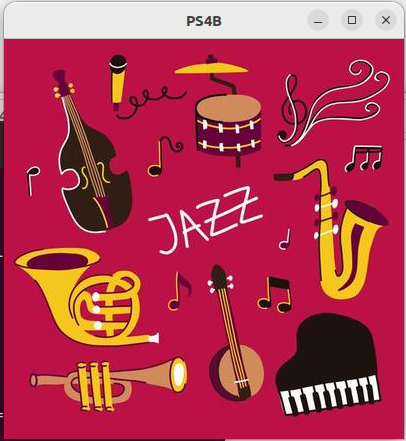
\includegraphics[width=0.69\textwidth]{ps4b/ps4b.png}
    \caption{PS4b Output Window}
    \label{fig:ps4b}
\end{figure}


\newpage
